\section{Concorrenza}

Un criterio per classificare i sistemi di gestione di basi di dati è il numero di utenti che possono
usare il sistema concorrentemente. Un sistema è \textbf{singolo-utente} se può essere usato da al più un
utente alla volta ed è \textbf{multiutente} se molti utenti possono usarlo contemporaneamente; la maggior
parte dei sistemi di gestione di basi di dati è del secondo tipo.\\
Se il sistema di calcolo ha più CPU allora è possibile il simultaneo processamento di due
programmi da parte di due diverse CPU; tuttavia la maggior parte della teoria del controllo della
concorrenza nelle basi di dati è stata sviluppata per sistemi di calcolo con una sola CPU. In tali
sistemi i programmi sono eseguiti concorrentemente in modo \emph{interleaved}, ovvero interfogliato: la CPU
può eseguire un solo programma alla volta, tuttavia il sistema operativo permette di eseguire alcune
istruzioni di un programma, sospendere quel programma, eseguire istruzioni di un altro programma
e quindi ritornare ad eseguire istruzioni del primo. In tal modo l'esecuzione concorrente dei
programmi è interleaved; ciò consente di tenere la CPU occupata quando un programma deve
effettuare operazioni di I/O.\\
\subsection{Scheduling di transazioni}
In un sistema di gestione di basi di dati multiutente la principale risorsa a cui i vari programmi
accedono concorrentemente è la base di dati. L'esecuzione di una parte di un programma che
rappresenta un'unità logica di accesso o modifica del contenuto della base di dati è detta
transazione. Ci sono sistemi (ad esempio le basi di dati statistici) in cui gli utenti effettuano solo
interrogazioni ma non modifiche; in tali sistemi l'esecuzione concorrente di più transazioni non crea
problemi. Al contrario nei sistemi in cui vengono effettuate da più utenti sia operazioni di lettura
che di scrittura (un tipico esempio di sistemi di questo tipo è costituito dai sistemi per la
prenotazione di posti sui voli) l'esecuzione concorrente di più transazioni può provocare problemi
se non viene controllata in qualche modo.\\
Prima di esaminare alcuni dei problemi che possono sorgere quando l'esecuzione concorrente di più
transazioni non è controllata, introduciamo il concetto di \textbf{schedule} (piano di esecuzione) di un
insieme di transazioni.
\begin{defn}
Dato un insieme $T$ di transazioni, uno \textbf{schedule} $S$ di $T$ è un ordinamento delle
operazioni nelle transazioni in $T$ tale che per ogni transazione $t$ in $T$ se $o_1$ e $o_2$ sono due operazioni
in $t$ tali che $o_1$ precede $o_2$ in $t$ allora $o_1$ precede $o_2$ in $S$.
\end{defn}
In altre parole uno schedule deve \emph{conservare l'ordine} che le operazioni hanno all'interno delle singole 
transazioni. Qualsiasi schedule ottenuto permutando le transazioni in $T$ è detto \emph{seriale}.
Consideriamo le seguenti transazioni

\begin{multicols}{2}  
 \begin{tabular}{|l|}
   \hline
   $t_1$\\
   \hline
   read(X)\\ 
   $X\vcentcolon=X-N$\\ 
   write(X)\\ 
   read(Y)\\
   $Y\vcentcolon=Y+N$\\
   write(Y)\\
   \hline
  \end{tabular} 
  
 \begin{tabular}{|l|}
  \hline
   $t_2$\\
   \hline
   read(X)\\ 
   $X\vcentcolon=X+M$\\ 
   write(X)\\
   \\
   \\
   \hline\\
  \end{tabular}
 \end{multicols}
 
 e i seguenti schedule di $\{t_1 ,t_2\}$:

 \begin{multicols}{2}  
 \begin{tabular}{|l|l|}
 \hline
 $t_1$ & $t_2$\\
 \hline
   read(X) & \\ 
   $X\vcentcolon=X-N$ & \\ 
   & read(X)\\
   & $X\vcentcolon=X+M$\\ 
   write(X) &\\ 
   read(Y) &\\
   & write(X)\\
   $Y\vcentcolon=Y+N$ &\\
   write(Y)&\\
   \hline
  \end{tabular}
  
  \begin{tabular}{|l|l|}
   \hline
   $t_1$ & $t_2$\\
   \hline
   read(X) & \\ 
   $X\vcentcolon=X-N$ & \\ 
   write(X) &\\ 
   & read(X)\\
   & $X\vcentcolon=X+M$\\ 
   & write(X)\\
   read(Y) &\\
   $Y\vcentcolon=Y+N$ &\\
   write(Y)&\\
   \hline
  \end{tabular}
  
  
 \end{multicols}

Nel primo caso l'aggiornamento di $X$ prodotto da $t_1$ viene perso in quanto $t_2$ legge il valore di $X$
prima che l'aggiornamento prodotto da $t_1$ sia stato reso permanente. Nel secondo caso $t_2$ legge e
aggiorna il valore di $X$ dopo che l'aggiornamento prodotto da $t_1$ è stato reso permanente, ma prima
che venga ripristinato il vecchio valore di $X$ in conseguenza del fallimento di $t_1$.\\

Consideriamo ora una transazione $t_3$ che somma i valori di $X$ e di $Y$. Il seguente schedule di
$\{t_1, t_3\}$ fa sì che la somma prodotta da $t_3$ sia la somma del valore di $X$ dopo che $X$ è stato
aggiornato da $t_1$ e del valore di $Y$ prima che sia stato aggiornato da $t_1$.
\begin{center}
  \begin{tabular}{|l|l|}
   \hline
   $t_1$ & $t_3$\\
   \hline
   & $somma\vcentcolon=0$\\
   read(X) & \\ 
   $X\vcentcolon=X-N$ & \\ 
   write(X) &\\ 
   & read(X)\\
   & $somma\vcentcolon=somma + X$\\ 
   & read(Y)\\
   & $somma\vcentcolon= somma + Y$\\
   read(Y) &\\
   $Y\vcentcolon=Y+N$ &\\
   write(Y)&\\
   \hline
  \end{tabular}
\end{center}
In tutti e tre i casi visti siamo portati a considerare gli schedule non corretti in quanto i valori
prodotti non sono quelli che si avrebbero se le due transazioni fossero eseguite nel modo ``naturale''
cioè sequenzialmente.\\
In generale possiamo osservare che l'esecuzione naturale e, quindi, intuitivamente corretta di un
insieme di transazioni è quella \emph{sequenziale}; la possibilità di eseguire concorrentemente un insieme
di transazioni, come si è detto, è introdotta nei sistemi per motivi di efficienza. Pertanto tutti gli
schedule seriali sono corretti e uno schedule non seriale è corretto se è \emph{serializzabile}, cioè se è
``\textbf{equivalente}'' ad uno schedule seriale. Sorge quindi la necessità di definire un concetto di
equivalenza di schedule.\\
La più semplice definizione di equivalenza potrebbe essere basata sul confronto del risultato: due
schedule sono equivalenti se producono lo stesso stato finale. Tale definizione non è però
soddisfacente in quanto due schedule potrebbero produrre lo stesso stato finale solo per alcuni
valori iniziali. Consideriamo ad esempio le due transazioni 
\begin{multicols}{2}  
 \begin{tabular}{|l|}
   \hline
   $t_1$\\
   \hline
   read(X)\\ 
   $X\vcentcolon=X+5$\\ 
   write(X)\\ 
   \hline
  \end{tabular}

  \begin{tabular}{|l|}
  \hline
   $t_2$\\
   \hline
   read(X)\\ 
   $X\vcentcolon=X*1.5$\\ 
   write(X)\\
   \hline
  \end{tabular}

 \end{multicols}

 e i seguenti schedule di $\{t_1 ,t_2\}$:
\begin{multicols}{2}  
 \begin{tabular}{|l|l|}
 \hline
 $t_1$ & $t_2$\\
 \hline
   read(X) & \\
   & read(X)\\
   $X\vcentcolon=X+5$ & \\ 
   & $X\vcentcolon=X*1.5$\\
   & write(X)\\ 
   write(X) &\\ 
   \hline
  \end{tabular}

  \begin{tabular}{|l|l|}
   \hline
   $t_1$ & $t_2$\\
   \hline
   read(X) & \\
   & read(X)\\
   & $X\vcentcolon=X*1.5$\\
   $X\vcentcolon=X+5$ & \\ 
   write(X) &\\   
   & write(X)\\
   \hline
  \end{tabular}
 \end{multicols}
 
Tali schedule producono gli stessi valori solo se il valore iniziale di $X$ è $10$; ma producono valori
diversi in tutti gli altri casi. Problemi di questo tipo potrebbero essere evitati sfruttando proprietà
algebriche che garantiscano che il risultato sia lo stesso indipendentemente dai valori iniziali delle
variabili; tuttavia tale soluzione richiederebbe dei costi inaccettabili (che non sono giustificati dallo
scopo che si vuole raggiungere). Pertanto si fa l'assunzione più restrittiva che due valori sono
uguali solo se sono prodotti da esattamente la stessa sequenza di operazioni. Quindi, ad esempio,
date le due transazioni

\begin{multicols}{2}  
 \begin{tabular}{|l|}
   \hline
   $t_1$\\
   \hline
   read(X)\\ 
   $X\vcentcolon=X+N$\\ 
   write(X)\\ 
   \hline
  \end{tabular}



  \begin{tabular}{|l|}
  \hline
   $t_2$\\
   \hline
   read(X)\\ 
   $X\vcentcolon=X-M$\\ 
   write(X)\\
   \hline
  \end{tabular}

 \end{multicols}

 e i due schedule:
\begin{multicols}{2}  
 \begin{tabular}{|l|l|}
 \hline
 $t_1$ & $t_2$\\
 \hline
   read(X) & \\
   $X\vcentcolon=X+N$&\\ 
   write(X)&\\ 
   &read(X)\\ 
   &$X\vcentcolon=X-M$\\ 
   &write(X)\\
   \hline
  \end{tabular}

  \begin{tabular}{|l|l|}
   \hline
   $t_1$ & $t_2$\\
   \hline
   &read(X)\\ 
   &$X\vcentcolon=X-M$\\ 
   &write(X)\\
   read(X) & \\
   $X\vcentcolon=X+N$&\\ 
   write(X)&\\ 
   \hline
  \end{tabular}
 \end{multicols}
 
non sono considerati equivalenti.\\

Oltre alla definizione di equivalenza, un altro elemento che ha influenza sulla complessità del
problema di decidere se uno schedule è serializzabile (cioè se è equivalente ad uno schedule seriale)
è costituito dal fatto che il valore calcolato da una transazione per ogni dato sia \emph{dipendente} o meno
dal vecchio valore di quel dato. Nel primo caso il problema della serializzabilità può essere risolto
in tempo polinomiale con un semplice algoritmo su grafi; nel secondo caso il problema risulta
essere \emph{NP-completo}.\\
Nella pratica è difficile testare la serializzabilità di uno schedule. Infatti l'ordine di esecuzione delle
operazioni delle diverse transazioni è determinato in base a diversi fattori: il carico del sistema,
l'ordine temporale in cui le transazioni vengono sottomesse al sistema e le loro priorità. Pertanto è
praticamente impossibile determinare in anticipo come le operazioni saranno interleaved, cioè in
quale ordine verranno eseguite; d'altra parte, se prima si eseguono le operazioni e poi si testa la
serializzabilità dello schedule, i suoi effetti devono essere annullati se lo schedule risulta non
serializzabile. Inoltre quando le transazioni vengono sottomesse al sistema in modo continuo è
difficile stabilire quando uno schedule comincia e quando finisce. Quindi l'approccio seguito nei
sistemi è quello di determinare metodi che garantiscano la serializzabilità di uno schedule
eliminando così la necessità di dover testare ogni volta la serializzabilità di uno schedule. Uno di
4tali metodi consiste nell'imporre dei protocolli, cioè delle regole, alle transazioni in modo da
garantire la serializzabilità di ogni schedule. Questi protocolli usano tecniche di \emph{locking} (cioè di
controllo dell'accesso ai dati) per prevenire l'accesso concorrente ai dati. Altri metodi di controllo
usano i \textbf{timestamp} delle transazioni, cioè degli identificatori delle transazioni che vengono generati
dal sistema e in base ai quali le operazioni delle transazioni possono essere ordinate in modo da
assicurare la serializzabilità.

\subsection{Item}
Tutte le tecniche per la gestione della concorrenza richiedono che la base di dati sia partizionata in
item, cioè in unità a cui l'accesso è controllato. Le dimensioni degli item devono essere definite in
base all'uso che viene fatto della base di dati in modo tale che in media una transazione acceda a
pochi item. Ad esempio se la transazione tipica su una base di dati relazionale è la ricerca di una
tupla mediante un indice, è appropriato trattare le tuple come item; se invece la transazione tipica
consiste nell'effettuazione di un join di due relazioni, è opportuno considerare le relazioni come
item. Le dimensioni degli item usate da un sistema sono dette la sua granularità. Una granularità
grande permette una gestione efficiente della concorrenza; una piccola granularità può invece
sovraccaricare il sistema, ma consente l'esecuzione concorrente di molte transazioni.

\subsection{Tecniche di locking per il controllo della concorrenza}
Queste tecniche fanno uso del concetto di lock. Un \textbf{lock} è un privilegio di accesso ad un singolo
item. In pratica è una variabile associata all'item il cui valore descrive lo stato dell'item rispetto alle
operazioni che possono essere effettuate su di esso. Un lock viene richiesto da una transazione
mediante un'operazione di locking e viene rilasciato mediante un'operazione di unlocking; fra
l'esecuzione di un'operazione di locking su un certo item $X$ e l'esecuzione di un'operazione di
unlocking su $X$ diciamo che la transazione mantiene un lock su $X$. Sono stati studiati diversi tipi di
lock; in ogni caso si assume che una transazione debba effettuare un'operazione di locking ogni
volta che deve leggere o scrivere un item e che l'operazione agisca come primitiva di
sincronizzazione, cioè se una transazione richiede un lock su un item su cui un'altra transazione
mantiene un lock, la transazione non può procedere finchè il lock non viene rilasciato dall'altra
transazione. Inoltre si assume che ciascuna transazione rilascia ogni lock che ha ottenuto. Uno
schedule è detto legale se obbedisce a queste regole.

\subsubsection{Lock binario}
Un \textbf{lock binario} può assumere solo due valori \emph{locked} e \emph{unlocked}. Le transazioni 
fanno uso di due operazioni \emph{lock(X)} e \emph{unlock(X)}; la prima serve per richiedere l'accesso
all'item $X$, la seconda per rilasciare l'item $X$ consentendone l'accesso ad altre transazioni. Se una 
transazione richiede l'accesso ad un item $X$ mediante un lock(X) e il valore della variabile è locked 
la transazione viene messa in attesa, altrimenti viene consentito alla transazione l'accesso ad $X$ e 
alla variabile associata ad $X$ viene assegnato il valore locked. 
Se una transazione rilascia un item $X$ mediante un unlock(X), alla variabile associata ad $X$ 
viene assegnato il valore unlocked; in tal modo se un'altra transazione è in attesa di accedere ad $X$ 
l'accesso gli viene consentito. Consideriamo di nuovo le due transazioni dell'esempio precedente e 
vediamo come l'uso dei lock può prevenire il problema dell'``aggiornamento perso''. 
Le transazioni $t_1$ e $t_2$ risultano modificate nel modo seguente 

\begin{multicols}{2}  

 \begin{tabular}{|l|}
   \hline
   $t_1$\\
   \hline
   lock(X)\\
   read(X)\\
   $X\vcentcolon=X-N$\\
   write(X)\\ 
   unlock(X)\\ 
   lock(Y)\\
   read(Y)\\
   $Y\vcentcolon=Y+N$\\
   write(Y)\\
   unlock(Y)\\
  \hline
 \end{tabular}
 
 \begin{tabular}{|l|}
  \hline
   $t_2$\\
   \hline
   lock(X)\\
   read(X)\\
   $X\vcentcolon=X+M$\\
   write(X)\\ 
   unlock(X)\\ 
  \\
  \\
  \\
  \hline
  \end{tabular}
  \\
 \end{multicols}

Uno schedule legale di $t_1$ e $t_2$ è il seguente:
\begin{center}
 \begin{tabular}{|l|l|}
 \hline
 $t_1$ & $t_2$\\
 \hline
   lock(X)&\\
   read(X)&\\
   $X\vcentcolon=X-N$&\\
   write(X)&\\ 
   unlock(X)&\\
   &lock(X)\\
   &read(X)\\
   &$X\vcentcolon=X+M$\\
   &write(X)\\ 
   &unlock(X)\\
   lock(Y)&\\
   read(Y)&\\
   $Y\vcentcolon=Y+N$&\\
   write(Y)&\\
   unlock(Y)&\\
   \hline
  \end{tabular}
\end{center}

Il più semplice modello per le transazioni è quello che considera una transazione come una
sequenza di operazioni di lock e unlock. Si assume che ogni operazione di lock su un item $X$ implica
la lettura di $X$ e ogni operazione di unlock di un item $X$ implica la scrittura di $X$. Il nuovo valore
dell'item viene calcolato da una funzione che è associata in modo univoco ad ogni coppia lockunlock
ed ha per argomenti tutti gli item letti (locked) dalla transazione prima dell'operazione di
unlock. I valori che un item assume durante l'esecuzione di una transazione sono formule costruite
applicando le funzioni suddette ai valori iniziali degli item. Due schedule sono equivalenti se le
formule che danno i valori finali per ciascun item sono le stesse per i due schedule.\\
Consideriamo ad esempio le due transazioni seguenti:

\begin{multicols}{2}  

 \begin{tabular}{|l|}
   \hline
   $t_1$\\
   \hline
   lock(X)\\ 
   unlock(X)$f_1$(X)\\ 
   lock(Y)\\ 
   unlock(Y)$f_2$(X,Y)\\ 
  \hline
 \end{tabular}
 
 \begin{tabular}{|l|}
  \hline
   $t_2$\\
   \hline
   lock(Y)\\
   unlock(Y)$f_3$(Y)\\
   lock(X)\\
   unlock(X)$f_4$(X,Y)\\
  \hline
  \end{tabular} 
 \end{multicols}

e il seguente schedule $S$ di $t_1$ e $t_2$:
\begin{center}
 \begin{tabular}{|l|l|}
 \hline
 $t_1$ & $t_2$\\
 \hline
   lock(X)&\\
   unlock(X)&\\
   &lock(Y)\\
   &unlock(Y)\\
   lock(Y)&\\ 
   unlock(Y)&\\
   &lock(X)\\
   &unlock(X)\\
   \hline
  \end{tabular}
\end{center}
Se indichiamo con $X_0$ e $Y_0$ i valori iniziali di $X$ e $Y$, abbiamo che il valore finale per $X$ prodotto da $S$
è dato dalla formula $f_4(f_1(X_0), Y_0)$. D'altra parte il valore finale per $X$ prodotto dallo schedule
seriale $t_1$, $t_2$ è dato dalla formula $f_4(f_1(X_0), f_2(X_0, Y_0))$, mentre il valore finale per $X$ prodotto dallo
schedule seriale $t_2$, $t_1$ è dato dalla formula $f_1(f_4(X_0, Y_0))$; pertanto $S$ non è serializzabile in quanto
non è equivalente a nessuno schedule seriale di $\{t_1, t_2\}$.\\

\noindent Consideriamo ora le due transazioni seguenti
\begin{multicols}{2}  

 \begin{tabular}{|l|}
   \hline
   $t_1$\\
   \hline
   lock(X)\\ 
   unlock(X)$f_1$(X)\\ 
   lock(Y)\\ 
   unlock(Y)$f_2$(X,Y)\\ 
  \hline
 \end{tabular}
 
 \begin{tabular}{|l|}
  \hline
   $t_2$\\
   \hline
   lock(X)\\
   unlock(X)$f_3$(X)\\
   lock(Y)\\
   unlock(Y)$f_4$(X,Y)\\
  \hline
  \end{tabular} 
 \end{multicols}

e il seguente schedule $S$ di $t_1$ e $t_2$:
\begin{center}
 \begin{tabular}{|l|l|}
 \hline
 $t_1$ & $t_2$\\
 \hline
   lock(X)&\\
   unlock(X)&\\
   &lock(X)\\
   &unlock(X)\\
   lock(Y)&\\ 
   unlock(Y)&\\
   &lock(Y)\\
   &unlock(Y)\\
   \hline
  \end{tabular}
\end{center}

Se di nuovo indichiamo con $X_0$ e $Y_0$ i valori iniziali di $X$ e $Y$, abbiamo che il valore finale per $X$ e $Y$
prodotti da $S$ sono dati rispettivamente dalle formule $f_3(f_1(X_0))$ e $f_4(f_1(X_0), f_2(X_0, Y_0))$. Poiché tali
formule coincidono con quelle prodotte dallo schedule seriale \{$t_1, t_2\}$, lo schedule S è serializzabile.\\

La serializzabilità di uno schedule in questo semplice modello, può essere testata mediante un
semplice algoritmo su grafi diretti. L'idea su cui si basa tale algoritmo è la seguente. Dato uno
schedule, per ogni item si esamina l'ordine in cui le varie transazioni fanno un lock su quell'item; se
lo schedule è serializzabile questo ordine deve essere consistente con quello di uno schedule seriale;
pertanto se l'ordine imposto sulle transazioni da un certo item è diverso da quello imposto da un
altro item, lo schedule non è serializzabile. L'algoritmo lavora nel modo seguente.

\begin{alg}
Dato uno schedule S:
\begin{itemize}
 \item crea un grafo diretto $G$ (grafo di serializzazione) i cui nodi corrispondono alle transazioni; in
tale grafo c'è un arco diretto da $t_i$ a $t_j$ se in $S$ $T_i$ esegue un $unlock(X)$ e $T_j$ esegue il successivo
$lock(X)$ (il significato intuitivo dell'esistenza di un arco da $t_i$ a $t_j$ è che $t_j$ legge il valore per $X$
scritto da $t_i$ e quindi se esiste uno schedule seriale equivalente ad $S$ in tale shedule $t_i$ deve
precedere $t_j$);
\item verifica se $G$ ha un ciclo. Se $G$ ha un ciclo allora $S$ non è serializzabile; altrimenti esiste un
ordinamento $S'$ delle transazioni tale che $t_i$ precede $t_j$ se c'è in $G$ un arco diretto da $T_i$ a $T_j$; tale
ordinamento può essere ottenuto applicando a $G$ il procedimento noto come ordinamento
topologico consistente nell'eliminare ricorsivamente da un grafo diretto i nodi che non hanno
archi entranti (l'ordine di eliminazione dei nodi fornisce lo schedule seriale $S'$).
\end{itemize}
\end{alg}

Il seguente teorema prova la correttezza dell'algoritmo.
\label{teorema_6_1}
\begin{theo}
L'Algoritmo 1 determina correttamente se uno schedule è serializzabile. 
\end{theo}
\textbf{Dimostrazione.} Cominciamo con il dimostrare che se il grafo di serializzazione $G$ contiene un ciclo allora $S$
non è serializzabile. Supponiamo, per assurdo, che $G$ contenga un ciclo $t_1$, $t_2, \ldots, t_k$, $t_1$ e che
esista uno schedule seriale $S'$ equivalente ad $S$. Sia $t_i$, $1\leq i \leq k$, la transazione del ciclo che compare
per prima in $S'$ e sia $X$ l'item che causa la presenza in $G$ dell'arco da $t_i-1$ a $t_i$. Il valore finale per $X$
prodotto da $S'$ è dato da una formula in cui compare una funzione $f$ associata ad una coppia lockunlock
in $t_i-1$ e almeno uno degli argomenti di $f$ è una formula in cui compare una funzione $g$
associata ad una coppia lock-unlock in $t_i$. D'altra parte in $S$ l'effetto di $t_i-1$ su $X$ precede quello di $t_i$
su $X$ ; quindi nella formula che dà il valore finale per $X$ prodotto da $S$ la funzione f compare più
internamente di $g$ ($f$ è applicata prima di $g$). Pertanto $S'$ ed $S$ non sono equivalenti (contraddizione).
Mostriamo ora che se $G$ non ha cicli allora $S$ è serializzabile. A tal fine definiamo profondità di una
transazione $t$ la lunghezza del più lungo cammino in $G$ da un qualsiasi nodo a $t$.
Sia $S'$ lo schedule seriale costruito dall'algoritmo; mostreremo per induzione sulla profondità delle
transazioni che ogni transazione $t$ per ogni item su cui effettua un'operazione di lock legge in $S$ lo
stesso valore che legge in $S'$ (e quindi per ogni item su cui effettua un'operazione di lock produce in
$S$ lo stesso valore che produce in $S'$).
Base dell'induzione. Se per una transazione $t$ la profondità è 0 vuol dire che in $G$ non ci sono archi
entranti in $t$; pertanto in $S$ $t$ legge solo valori iniziali. D'altra parte in $S'$ $t$ viene prima di qualsiasi
transazione che effettua un'operazione di lock su un item su cui $t$ effettua un'operazione di lock.
Infatti, se $X$ è un item su cui $t$ effettua un'operazione di lock e $t_{i_1}, t_{i_2}, \ldots, t_{i_k}$ è la sequenza in $S$
delle transazioni che effettuano un'operazione di lock su $X$, $t_{i_1}, t_{i_2}, \ldots, t_{i_k}$ è un cammino in $G$;
poiché $t$ deve comparire in tale cammino e in $G$ non ci sono archi entranti in $t$, si deve avere $t=t_{i_1}$
e quindi nessun altro nodo del cammino può essere eliminato dal procedimento di ordinamento
topologico prima di $t$.
Induzione. Cominciamo con il mostrare che ogni transazione per ogni item su cui effettua
un'operazione di lock legge sia in $S$ che in $S'$ il valore prodotto da una stessa transazione.
Supponiamo, per assurdo, che esistano una transazione $t$ e un item $X$ tali che $t$ legge in $S$ il valore
di $X$ prodotto da una transazione $t'$ e in $S'$ il valore prodotto da un'altra transazione $t''$. Sia $t_{i_1},
t_{i_2}, \ldots, t_{i_k}$ la sequenza in $S$ delle transazioni che effettuano un'operazione di lock su $X$; $t_{i_1},
t_{i_2}, \ldots, t_{i_k}$ è un cammino in $G$ in cui $t'$ compare immediatamente prima di $t$. Anche $t''$ compare in tale
cammino, e quindi deve comparire prima di $t'$. Poiché in $S'$, $t''$ deve seguire $t'$, $S'$ non può essere
ottenuto da $G$ mediante il procedimento di ordinamento topologico (contraddizione).
Sia $t$ una transazione che ha profondità $d$, $d>0$, in $G$; per quanto visto $t$, per ogni item su cui
effettua un'operazione di lock, legge sia in $S$ che in $S'$ il valore prodotto da una stessa transazione
$t'$. Poiché $t'$ ha profondità minore di $d$ per l'ipotesi induttiva $t'$, per ogni item su cui effettua
un'operazione di lock, legge sia in $S$ che in $S'$ lo stesso valore e, quindi, produce sia in $S$ che in $S'$ lo
stesso valore. Pertanto $t$, per ogni item su cui effettua un'operazione di lock, legge sia in $S$ che in $S'$
lo stesso valore. \hfill $\Box$\\
\begin{defn}
Diciamo che una transazione obbedisce al protocollo di locking a due fasi, o più semplicemente che
è \textbf{a due fasi}, se prima effettua tutte le operazioni di lock (fase di locking) e poi tutte le operazioni di
unlock (fase di unlocking). 
\end{defn}
Mostreremo che il protocollo di locking a due fasi garantisce la serializzabilità; più precisamente, si ha che:
\begin{theo}
Sia $T$ un insieme di transazioni. Se ogni transazione in $T$ è a due fasi allora ogni
schedule di $T$ è serializzabile. 
\end{theo}
\texbf{Dimostrazione.} Sia $S$ uno schedule di $T$. Supponiamo, per assurdo, che $S$ non sia serializzabile. Per il
\linkto{teorema_6_1}{Teorema 6.1}, il grafo di serializzazione $G$ di $S$ contiene un ciclo $t_{i_1}, t_{i_2}, \ldots,
t_{i_k}$; ciò significa che $T_{i+1}$, $i\in \{1,\ldots k-1\}$, effettua un'operazione di lock, su un item su cui $t_i$
ha effettuato un'operazione di unlock e che $t_1$ effettua un'operazione di lock, su un item su cui $t_k$ ha effettuato
un'operazione di unlock. Pertanto in $S$ $t_1$ effettua un'operazione di lock dopo aver effettuato un'operazione di unlock
e quindi $t_1$ non è a due fasi (contraddizione).\\

Mostreremo ora che se una transazione $t_1$ non è a due fasi, esiste sempre una transazione $t_2$ tale
che esiste uno schedule di $\{t_1, t_2\}$ che non è serializzabile. Infatti, se $t_1$ non è a due fasi, effettua
un'operazione di lock dopo aver effettuato un'operazione di unlock; consideriamo anche la seguente transazione $t_2$  

\begin{multicols}{2}  

 \begin{tabular}{|l|}
   \hline
   $t_1$\\
   \hline
   $\ldots$\\
   unlock(X)\\ 
   $\ldots$\\
   lock(Y)\\ 
   $\ldots$\\
  \hline
 \end{tabular}
 
 \begin{tabular}{|l|}
  \hline
   $t_2$\\
   \hline
   lock(X)\\
   lock(Y)\\
   unlock(X)\\
   unlock(Y)\\
  \hline
  
  \end{tabular} 
 \end{multicols}

 il seguente schedule $S$ di $t_1$ e $t_2$ non è serializzabile
\begin{center}
 \begin{tabular}{|l|l|}
 \hline
 $t_1$ & $t_2$\\
 \hline
   $\ldots$&\\
   unlock(X)&\\
   $\ldots$&\\
   &lock(X)\\
   &lock(Y)\\
   &unlock(X)\\    
   unlock(Y)&\\
   $\ldots$&\\
   &lock(Y)\\
   $\ldots$&\\
   \hline
  \end{tabular}
\end{center}

Infatti il suo grafo di serializzazione
\begin{center}
  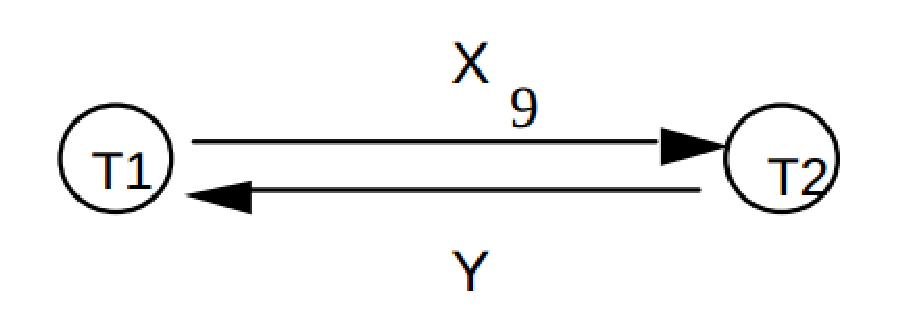
\includegraphics[width=150px]{img_6_3_1.eps}
\end{center}
contiene un ciclo. Naturalmente possono esistere schedule di transazioni che non sono a due fasi
che sono serializzabili. Tuttavia poiché è normale non conoscere l'insieme di transazioni con cui
una transazione può essere eseguita concorrentemente siamo costretti a richiedere che tutte le
transazioni siano a due fasi perché sia garantita la serializzabilità di ogni schedule.

\subsubsection{Lock a tre valori}
Consideriamo ora un modello per le transazioni che consente un maggior grado di concorrenza. In
tale modello si fa l’assunzione realistica che una transazione possa accedere ad un item solo per
leggerlo, senza modificarlo. Se una transazione desidera solo leggere un item $X$ effettua
un’operazione $rlock(X)$ che impedisce a qualsiasi altra transazione di modificare il valore di $X$;
tuttavia un qualsiasi numero di transazioni può ottenere contemporaneamente un lock di lettura su
$X$. Se, invece, una transazione desidera modificare il valore di $X$ effettua un’operazione $wlock(X)$; in
tal caso nessuna altra transazione può ottenere un lock di scrittura o di lettura su $X$. Entrambi i lock
sono rilasciati mediante un’operazione di $unlock(X)$. Pertanto si fa uso di un lock a tre valori:
$rlocked$, $wlocked$, $unlocked$.\\
Quanto detto per gli schedule legali vale anche in questo modello con l’unica differenza che una
transazione che mantiene un lock di lettura su un certo item può richiedere un lock in scrittura su
quello stesso item.\\
Analogamente a quanto fatto per il modello precedente assumiamo che quando una transazione
effettua un $wlock$ su un item il nuovo valore dell’item viene calcolato da una funzione,
univocamente associata a quell’operazione di $wlock$, che ha come argomenti tutti gli item su cui la
transazione ha già effettuato un lock (di lettura o di scrittura) prima dell’unlock associato al $wlock$.
Quindi, analogamente a quanto accadeva nel modello precedente, l’effetto di uno schedule sulla
base di dati può essere espresso dalle formule che calcolano (a partire dai valori iniziali degli item e
applicando le funzioni associate ai $wlock$) i valori degli item che sono modificati da almeno una
transazione. Tuttavia, poiché in questo modello si assume che una transazione possa leggere un item
senza modificarlo, la definizione di equivalenza di schedule deve essere modificata per tener conto
di tale eventualità.\\
\begin{defn}
 Due schedule sono \textbf{equivalenti} se:
 \begin{enumerate}
  \item producono lo stesso valore per ogni item su cui viene effettuato un wlock
  \item ogni operazione rlock(X) legge lo stesso valore di X nei due schedule.
 \end{enumerate}
\end{defn}


Vediamo ora quali condizioni di precedenza tra transazioni è possibile inferire dalla semantica delle
transazioni appena vista.\\
Supponiamo che in uno schedule $S$ una transazione $t_1$ effettui un’operazione $wlock$ su un item $X$ e
che una transazione $t_2$ effettui un’operazione rlock su $X$ prima che una terza transazione $t_3$ esegua
la successiva operazione di $wlock$ su $X$ (in altre parole, $t_1$ modifica il valore di $X$ e $t_2$ legge il
valore di $X$ prodotto da $t_1$ prima che $X$ venga nuovamente modificato da $t_3$). Allora in qualsiasi
schedule seriale equivalente ad S $t_1$ deve precedere $t_2$ e $t_2$ deve precedere $t_3$. D’altra parte, se due
transazioni $t_1$ e $t_2$ leggono entrambe il valore di un item $X$ prodotto da una transazione non è lecito
stabilire nessuna precedenza tra $t_1$ e $t_2$ .
Per rappresentare le precedenze tra le transazioni è possibile usare, come per il modello precedente,
un grafo diretto che ha per nodi le transazioni e ha un arco da una transazione $t_i$ a una transazione
$t_j$ se la semantica delle transazioni impone che $t_i$ debba precedere $t_j$. Analogamente a quanto
accade per il modello precedente, un semplice algoritmo su tale grafo permette di decidere se uno
schedule è serializzabile e in caso affermativo di ottenere uno schedule seriale equivalente ad esso.

\begin{alg}
Dato uno schedule $S$
\begin{itemize}
 \item crea un grafo diretto $G$ (grafo di serializzazione) i cui nodi corrispondono alle transazioni; in
tale grafo c’è un arco diretto da $t_i$ a $t_j$ se
 \begin{itemize}
  \item in $S$ $t_i$ esegue una $rlock(X)$ o una $wlock(X)$ e $t_j$ è la transazione che esegue la successiva
   $wlock(X)$
  \item in $S$ $t_i$ esegue una $wlock(X)$ e $t_j$ esegue una $rlock(X)$ dopo che $t_i$ ha eseguito la $wlock(X)$ e
prima che un’altra transazione esegua una $wlock(X)$.
 \end{itemize}
\item verifica se $G$ ha un ciclo. Se $G$ ha un ciclo allora $S$ non è serializzabile; altrimenti esiste un
ordinamento $S'$ delle transazioni tale che $t_i$ precede $t_j$ se c’è in $G$ un arco diretto da $t_i$ a $t_j$; tale
ordinamento può essere ottenuto applicando a $G$ il procedimento di ordinamento topologico.
\end{itemize}
\end{alg}

Il seguente teorema, che può essere dimostrato con la stessa tecnica usata per il \linkto{teorema_6_1}{Teorema 6.1},
prova la correttezza dell’algoritmo.
\begin{theo}
L’Algoritmo 2 determina correttamente se uno schedule è serializzabile. 
\end{theo}

